\documentclass[a4paper,12pt]{article} % добавить leqno в [] для нумерации слева
\usepackage[a4paper,top=1.3cm,bottom=2cm,left=1.5cm,right=1.5cm,marginparwidth=0.75cm]{geometry}
%%% Работа с русским языком
\usepackage{cmap}					% поиск в PDF
\usepackage[warn]{mathtext} 		% русские буквы в фомулах
\usepackage[T2A]{fontenc}			% кодировка
\usepackage[utf8]{inputenc}			% кодировка исходного текста
\usepackage[english,russian]{babel}	% локализация и переносы
\usepackage{physics}
\usepackage{multirow}
\usepackage{longtable}

%%% Нормальное размещение таблиц (писать [H] в окружении таблицы)
\usepackage{float}
\restylefloat{table}



\usepackage{graphicx}

\usepackage{wrapfig}
\usepackage{tabularx}

\usepackage{hyperref}
\usepackage[rgb]{xcolor}
\hypersetup{
	colorlinks=true,urlcolor=blue
}

\usepackage{pgfplots}
\pgfplotsset{compat=1.9}

%%% Дополнительная работа с математикой
\usepackage{amsmath,amsfonts,amssymb,amsthm,mathtools} % AMS
\usepackage{icomma} % "Умная" запятая: $0,2$ --- число, $0, 2$ --- перечисление

%% Номера формул
\mathtoolsset{showonlyrefs=true} % Показывать номера только у тех формул, на которые есть \eqref{} в тексте.

%% Шрифты
\usepackage{euscript}	 % Шрифт Евклид
\usepackage{mathrsfs} % Красивый матшрифт

%% Свои команды
\DeclareMathOperator{\sgn}{\mathop{sgn}}

%% Перенос знаков в формулах (по Львовскому)
\newcommand*{\hm}[1]{#1\nobreak\discretionary{}
	{\hbox{$\mathsurround=0pt #1$}}{}}

\date{\today}

\usepackage{gensymb}

\begin{document}

\begin{titlepage}
    \begin{center}
         \footnotesize{ФЕДЕРАЛЬНОЕ ГОСУДАРСТВЕННОЕ АВТОНОМНОЕ ОБРАЗОВАТЕЛЬНОЕ \\УЧРЕЖДЕНИЕ ВЫСШЕГО ОБРАЗОВАНИЯ}\\
    \footnotesize{МОСКОВСКИЙ ФИЗИКО-ТЕХНИЧЕСКИЙ ИНСТИТУТ\\(НАЦИОНАЛЬНЫЙ 			ИССЛЕДОВАТЕЛЬСКИЙ УНИВЕРСИТЕТ)}\\
    \footnotesize{ФИЗТЕХ-ШКОЛА РАДИОТЕХНИКИ И КОМПЬЮТЕРНЫХ ТЕХНОЛОГИЙ\\}
    \end{center}
    \vspace*{5cm}
	{\huge
		\begin{center}
		
			{  Отчёт по лабораторной работе: }\\
			\bf3.6.1 Спектральный анализ электрических сигналов(компьютерная установка)
		\end{center}
	}
	\vspace{1cm}
	\begin{flushright}
		{\LARGE Автор:\\ Денишева Р.Р\\
			\vspace{0.2cm}
			Группа Б01-101}
	\end{flushright}
	\vspace{7cm}
	\begin{center}
		Долгопрудный\\
		\today
	\end{center}
\end{titlepage}


\section{Аннотация}

В работе изучается спектральный состав периодических электрических сигналов различной формы: последовательности прямоугольных импульсов, последовательности цугов и амплитудно модулированных гармонических колебаний. Спектры этих сигналов наблюдаются с помощью промышленного анализатора спектра и сравниваются с рассчитанными теоретически. 

\section{Теоретические сведения}

Сколь угодно сложный электрический сигнал V (t) может быть разложен на более простые сигналы. В радиотехнике широко используется разложение сигнала V (t) на совокупность гармонических сигналов различных частот $\omega$. Функция F($\omega$), описывающая зависимость амплитуд отдельных гармоник от частоты, называется амплитудной спектральной характеристикой сигнала V (t). Представление сложного периодического сигнала в виде суммы дискретных гармонических сигналов в математике называется разложением в ряд Фурье.

Зная спектральный состав F($\omega$) периодической последовательности некоторого импульса V (t), мы можем осуществить обратное преобразование Фурье: сложив отдельные гармоники со своими амплитудами и фазами, получить необходимую последовательность импульсов. Степень совпадения полученного сигнала с V (t) определяется количеством синтезированных гармоник: чем их больше, тем лучше совпадение.

Рассмотрим конкретные примеры периодических функций, которые будут предметом исследования в нашей работе.

\subsection{Спектральный анализ электрических сигналов}

\begin{center}
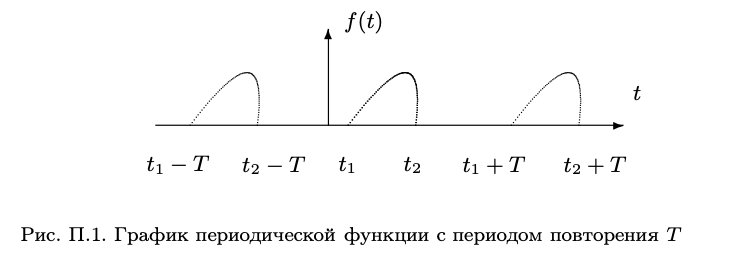
\includegraphics[width=0.7\linewidth]{1.jpeg}\\
\end{center}

Пусть заданная функция $f(t)$ периодически повторяется с частотой $\Omega_{1}=2 \pi / T,$ где $T-$ период повторения $($ рис. $\Pi .1) .$ Её разложение в ряд Фурье имеет вид
$$
f(t)=\frac{a_{0}}{2}+\sum_{n=1}^{\infty}\left[a_{n} \cos \left(n \Omega_{1} t\right)+b_{n} \sin \left(n \Omega_{1} t\right)\right]
$$
или
$$
f(t)=\frac{A_{0}}{2}+\sum_{n=1}^{\infty} A_{n} \cos \left(n \Omega_{1} t-\psi_{n}\right)
$$
Здесь $a_{0} / 2=A_{0} / 2-$ постоянная составляюпдая (среднее значение) функции $f(t) ; a_{n}$ и $b_{n}-$ амплитуды косинусных и синусных членов разложе-ния. Они определяются выражениями
$$
\begin{array}{l}
a_{n}=\frac{2}{T} \int_{t_{1}}^{t_{1}+T} f(t) \cos \left(n \Omega_{1} t\right) d t \\
b_{n}=\frac{2}{T} \int_{t_{1}}^{t_{1}+T} f(t) \sin \left(n \Omega_{1} t\right) d t
\end{array}
$$

Точку начала интегрирования $t_1$ можно выбрать произвольно.
В тех случаях, когда сигнал чётен относительно t = 0, в тригонометрической записи остаются только косинусные члены, т.к. все коэффициенты $b_n$ обращаются в нуль. Для нечётной относительно t = 0 функции, наоборот, ряд состоит только из синусных членов.

Амплитуда $A_{n}$ и фаза $\psi_{n} n$ -й гармоники выражаются через $a_{n}$ и $b_{n}$ следуюшим образом:
$$
A_{n}=\sqrt{a_{n}^{2}+b_{n}^{2}} ; \quad \psi_{n}=\operatorname{arctg} \frac{b_{n}}{a_{n}}
$$
Как мы видим, спектр любой периодической функции состоит из набора гармонических колебаний с дискретными частотами: $\Omega_{1}, 2 \Omega_{1}, 3 \Omega_{1}$ $\ldots$ и постоянной составляющей, которую можно рассматривать как колебание с нулевой частотой $\left(0 \cdot \Omega_{1}\right) .$

Представим выражение в комплексной форме. Для этого заменим косинусы экспонентами в соответствии с формулой
$$
\cos \alpha=\frac{e^{i \alpha}+e^{-i \alpha}}{2}
$$
Подстановка даёт
$$
f(t)=\frac{1}{2}\left(A_{0}+\sum_{n=1}^{\infty} A_{n} e^{-i \psi_{n}} e^{i n \Omega_{1} t}+\sum_{n=1}^{\infty} A_{n} e^{i \psi_{n}} e^{-i n \Omega_{1} t}\right)
$$
Введём комплексные амплитуды $\tilde{A}_{n}$ и $\tilde{A}_{-n}$

$$
\tilde{A}_{n}=A_{n} e^{-i \psi_{n}} ; \quad \tilde{A}_{-n}=A_{n} e^{i \psi_{n}} ; \quad \tilde{A}_{0}=A_{0}
$$
Разложение $f(t)$ приобретает вид
$$
f(t)=\frac{1}{2} \sum_{n=-\infty}^{\infty} \tilde{A}_{n} e^{i n \Omega_{1} t}
$$

Как мы видим, введение отрицательных частот (типа −n$\Omega_1$) позволяет записать разложение Фурье особенно простым образом. 

Для расчёта комплексных амплитуд $A_{n}$ yмножим левую и правую части на $e^{-i k \Omega_{1} t}$ и проинтегрируем полученное равенство по времени на отрезке, равном одному периоду, например, от $t_{1}=0$ до $t_{2}=2 \pi / \Omega_{1} .$ В правой части обратятся в нуль все члены, кроме одного, соответствующего $n=k .$ Этот член даёт $A_{k} T / 2 .$ Имеем поэтому
$$
A_{k}=\frac{2}{T} \int_{0}^{T} f(t) e^{-i k \Omega_{1} t} d t
$$
Рассмотрим периодические функции, которые исследуются в нашей paбoтe.


\subsection{Периодическая последовательность прямоугольных импульсов}
C амплитудой $V_{0},$ длительностью $\tau,$ частотой повторения $f_{\text {повт }}=1 / T,$ где $T-$ период повторения импульсов.


Cреднее значение


\langle V\rangle=\frac{a_{0}}{2}=\frac{A_{0}}{2}=\frac{1}{T} \int_{-\tau / 2}^{\tau / 2} V_{0} d t=V_{0} \frac{\tau}{T}

Амплитуды косинусных составляющих равны
$$
a_{n}=\frac{2}{T} \int_{-\tau / 2}^{\tau / 2} V_{0} \cos \left(n \Omega_{1} t\right) d t=2 V_{0} \frac{\tau}{T} \frac{\sin \left(n \Omega_{1} \tau / 2\right)}{n \Omega_{1} \tau / 2} \sim \frac{\sin x}{x}
$$
Поскольку наша функция чётная, все амплитуды синусоидальных гармоник $b_{n}=0 .$ Спектр $F(\nu)$ последовательности прямоугольных импульсов представлен на рис. П.3. Амплитуды гармоник $A_{n}$ меняются по Закону $(\sin x) / x$
На рис. П.3 изображён спектр для случая, когда $T$ кратно $\tau .$ Назовём шириной спектра $\Delta \omega$ (или $\Delta \nu$ ) расстояние от главного максимума $(\nu=0)$ до первого нуля, возникающего, как нетрудно убедиться, при $\Omega_{1}=2 \pi / \tau$ При этом
$$
\Delta \omega \tau \simeq 2 \pi \quad \text { или } \quad \Delta \nu \Delta t \simeq 1
$$
Полученное соотношение взаимной связи интервалов $\Delta \nu$ и $\Delta t$ является
частным случаем соотношения неопределенности в квантовой механике. Несовместимость острой локализации волнового процесса во времени с узким спектром частот - явление широко известное в радиотехнике. Ширина селективной настройки $\Delta \nu$ радиоприёмника ограничивает приём радиосигналов Длительностью $t<1 / \Delta \nu$

 \begin{center}
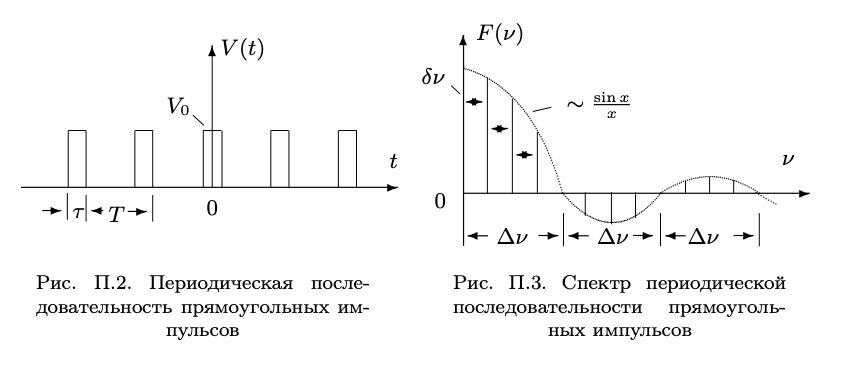
\includegraphics[width=0.7\linewidth]{2.jpeg}\\
\end{center}

\subsection{Периодическая последовательность цугов}
Гармонического колебания $V_{0} \cos \left(\omega_{0} t\right)$ с длительностью цуга $\tau$ и периодом повторения $T$ (рис. $\Pi .4)$
 
Функция $f(t)$ снова является чётной относительно $t=0 .$ Амплитуда $n$ -й гармоники равна
$$
\begin{array}{c}
A_{n}=a_{n}=\frac{2}{T} \int_{-\tau / 2}^{\tau / 2} V_{0} \cos \left(\omega_{o} t\right) \cdot \cos \left(n \Omega_{1} t\right) d t= \\
=V_{0} \frac{\tau}{T}\left(\frac{\sin \left[\left(\omega_{0}-n \Omega_{1}\right) \frac{\tau}{2}\right]}{\left(\omega_{0}-n \Omega_{1}\right) \frac{\tau}{2}}+\frac{\sin \left[\left(\omega_{0}+n \Omega_{1}\right) \frac{\tau}{2}\right]}{\left(\omega_{0}+n \Omega_{1}\right) \frac{\tau}{2}}\right)
\end{array}
$$

Такое спектральное распределение F ($\omega$) для случая, когда $\frac T\tau$ равно целому числу, представлено на рис. П.5. Сравнивая спектр последовательности прямоугольных импульсов и спектр цугов (см. рис. П.3 и П.5), мы видим, что они аналогичны, но их максимумы сдвинуты по частоте на величину $\omega_0$.

\begin{center}
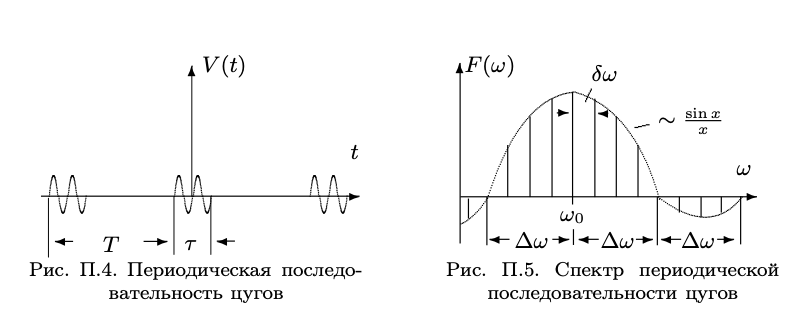
\includegraphics[width=0.7\linewidth]{3.jpeg}\\
\end{center}

\subsection{Амплитудно-модулированные колебания.}

\begin{center}
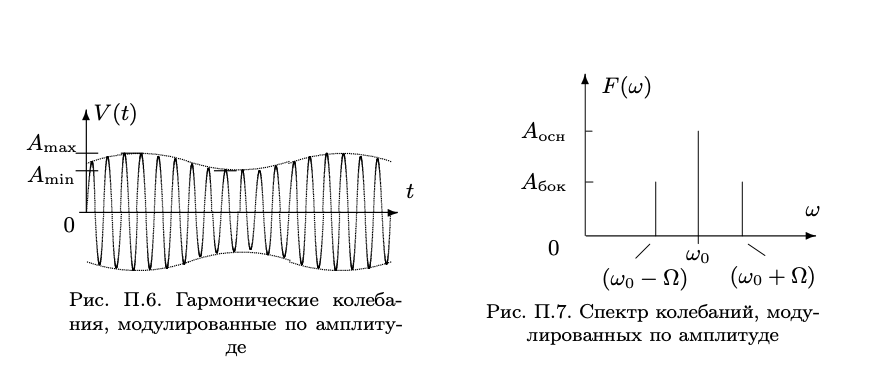
\includegraphics[width=0.7\linewidth]{4.jpeg}\\
\end{center}
 Рассмотрим гармонические колебания высокой частоты $\omega_{0},$ амплитуда которых медленно меняется по гармоническому закону с частотой $\Omega\left(\Omega \ll \omega_{0}\right)$ (рис. П.6):
$$
f(t)=A_{0}[1+m \cos (\Omega t)] \cos (\omega t)
$$
Коэффициент $m$ называют глубиной модуляции. При $m<1$ амплитуда колебаний меняется от минимальной $A_{\min }=A_{0}(1-m)$ до максимальной $A_{\max }=A_{0}(1+m) .$ Глубина модулящии может быть представлена в виде
$$
m=\frac{A_{\max }-A_{\min }}{A_{\max }+A_{\min }}
$$
Простым тригонометрическим преобразованием можно найти спектр амплитудно-модулированных колебаний:
$$
\begin{aligned}
f(t) &=A_{0} \cos \left(\omega_{0} t\right)+A_{0} m \cos (\Omega t) \cos \left(\omega_{0} t\right)=\\
=A_{0} \cos \left(\omega_{0} t\right) &+\frac{A_{0} m}{2} \cos \left(\omega_{0}+\Omega\right) t+\frac{A_{0} m}{2} \cos \left(\omega_{0}-\Omega\right) t
\end{aligned}
$$

Спектр $F(\omega)$ таких колебаний содержит три составляюшцих (рис. П. 7$)$ Основная компонента представляет собой исходное немодулированное колебание с иесущей частотой $\omega_{0}$ и амплитудой $A_{\mathrm{ocн}}=A_{0}-$ первое слагаемое в правой части; боковые компоненты спектра соответствуют гармоническим колебаниям с частотами $\left(\omega_{0}+\Omega\right)$ и $\left(\omega_{0}-\Omega\right)-$ Второе и третье слагаемые. Амплитуды этих двух колебаний одинаковы и составляют $m / 2$ от амплитуды немодулированного колебания: $A_{\text {бок }}=A_{0} m / 2$
\newpage

\section{Результаты измерений и обработка данных}
\subsection{Спектры прямоугольных импульсов}
Проанализируем, как меняется спектр 

a) при увеличении $\tau$ вдвое при неизменном $f_{\text {повт }}=1$ кГц. ширина основной части спектра уменьшилась в 2 раза\\

\begin{minipage}{0.44\textwidth}
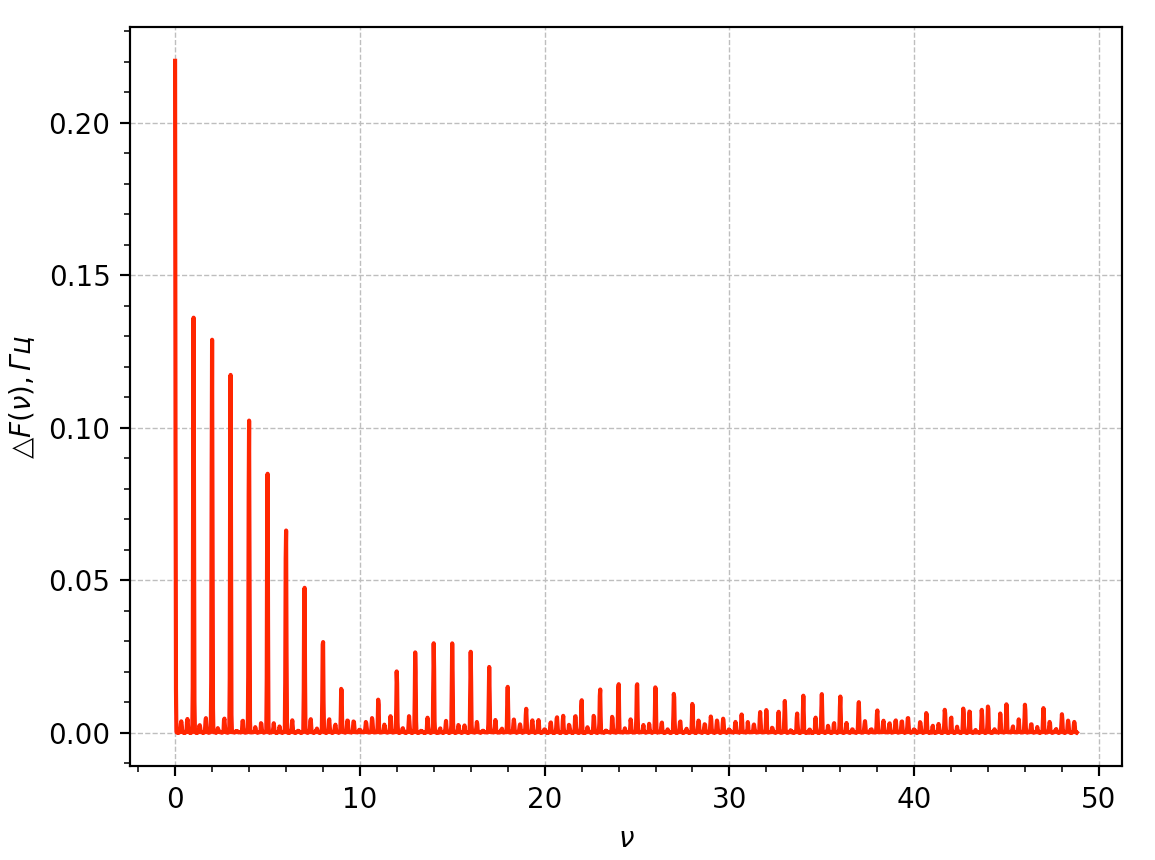
\includegraphics[width=\linewidth]{1.png}\\
\begin{center}
Рис.8 "Эталонный спектр"
\end{center}
\end{minipage}
\begin{minipage}{0.1\textwidth}
\ \ \ \ \ \ \Rightarrow
\end{minipage}
\begin{minipage}{0.44\textwidth}
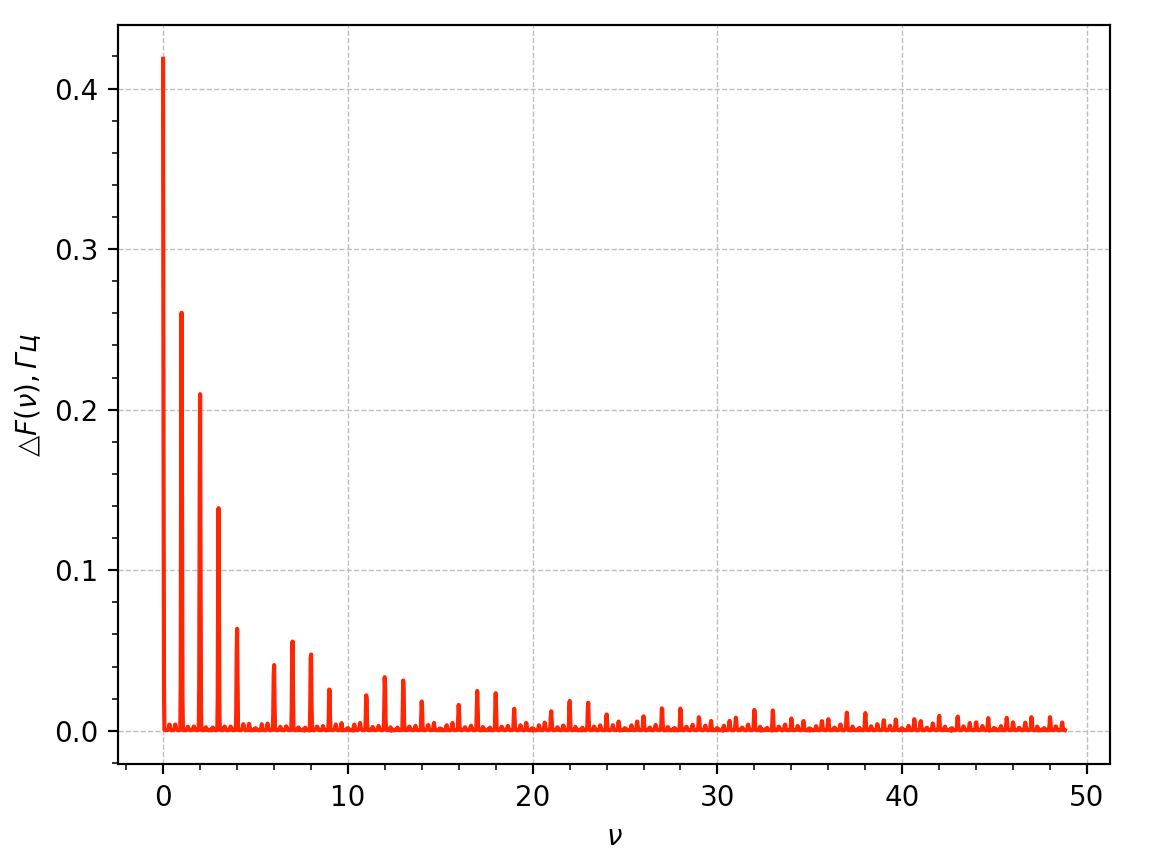
\includegraphics[width=\linewidth]{2.png}\\
\begin{center}
Рис.9 "Увеличение $\tau$ вдвое"
\end{center}
\end{minipage}

\\
\
\\
\

б) при увеличении $f_{\text {повт }}$ вдвое при неизменном $\tau=100$ мкс. уменьшилось в 2 раза количество гармоник. 

\begin{minipage}{0.44\textwidth}
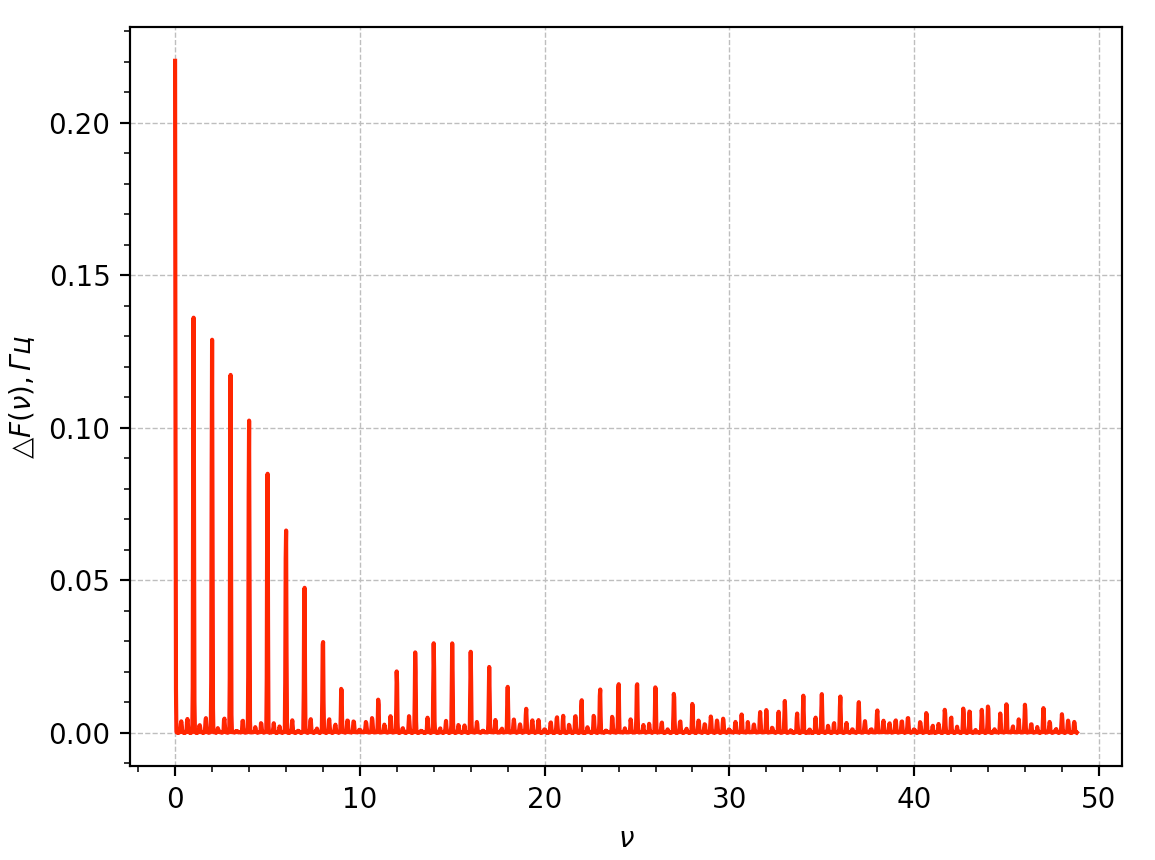
\includegraphics[width=\linewidth]{1.png}\\
\begin{center}
Рис.10 "Эталонный спектр"
\end{center}
\end{minipage}
\begin{minipage}{0.1\textwidth}
\ \ \ \ \ \ \Rightarrow
\end{minipage}
\begin{minipage}{0.44\textwidth}
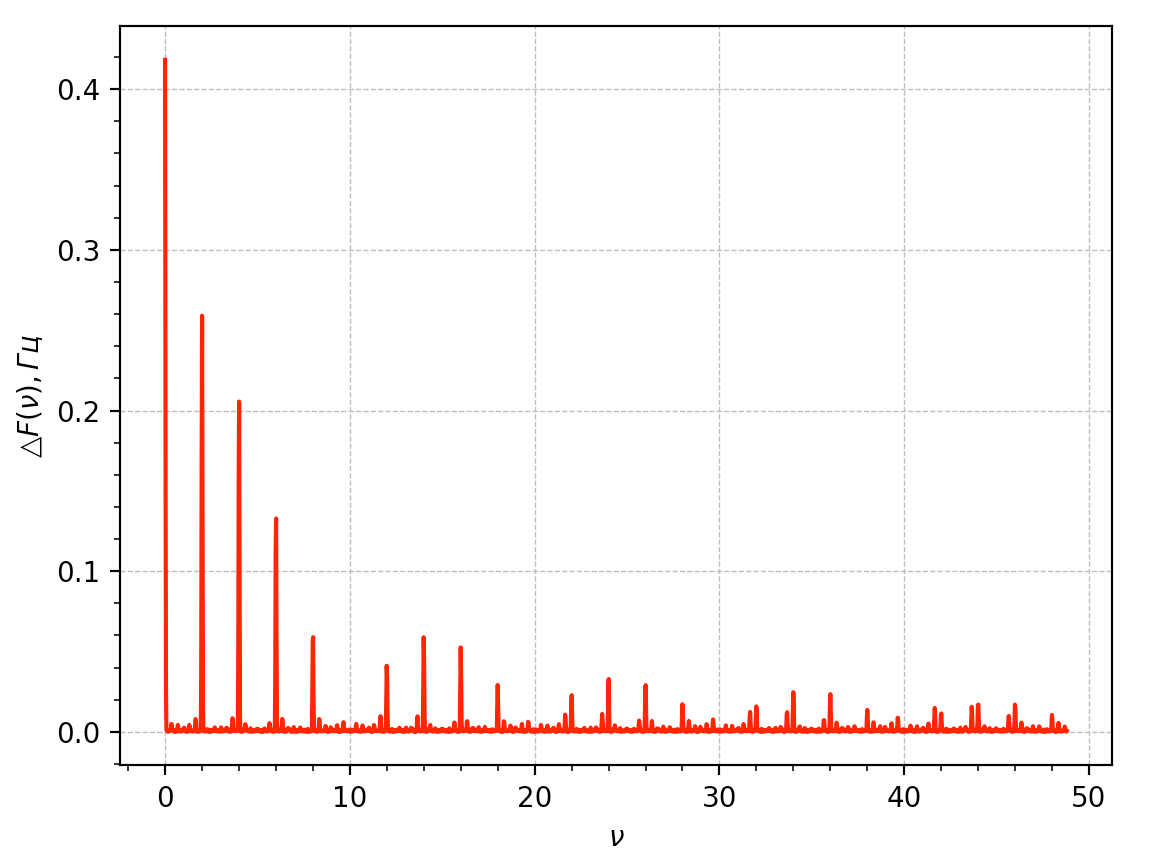
\includegraphics[width=\linewidth]{3.png}\\
\begin{center}
Рис.11 "Увеличение $f_{повт}$ вдвое"
\end{center}
\end{minipage}

\\
\
\\
\

Изучим зависимость $ \Delta \nu (\tau) $. Результат в таблице \ref{tab:nu-tau}.
\begin{table}[h]
	\centering
	\begin{tabular}{|l|l|l|l|l|l|l|l|l|l|}
		\hline
		${\tau}$      & 40    & 60    & 80    & 100   & 120  & 140  & 160  & 180  & 200  \\ \hline
		${\Delta \nu}$ & 25000 & 16000 & 12500 & 10000 & 9500 & 7000 & 6000 & 5500 & 5000 \\ \hline
	\end{tabular}
	\caption{Зависимость $\Delta \nu (\tau)$}
	\label{tab:nu-tau}
\end{table}

Построим картины спектров для $ \tau  =  50\; мкс $ (рис. 12) и $ \tau = 100\; мкс $ (рис. 13).

\begin{figure}[p]
	\centering
	\includegraphics[width=0.8\linewidth]{"50"}
                     \begin{center}
                    {Рис 12.} Картина спектра прямоугольного сигнала при $\tau = 50$ мкс\\
                    \end{center}

	\label{fig:1-50}
\end{figure}

\begin{figure}[p]
	\centering
	\includegraphics[width=0.8\linewidth]{"100"}
 \begin{center}
                    {Рис 13.} Картина спектра прямоугольного сигнала при $\tau = 100$ мкс\\
                    \end{center}
	\label{fig:1-100}
\end{figure}

Проверим справедливость соотношения неопределённостей. Для этого построим график $\nu(1/\tau)$(рис.14)

\begin{center}
                    \begin{tikzpicture}
                        \begin{axis}[
                            title =  $ \Delta \nu (1/\tau) $ ,
                            grid = major,
                            height = 0.25\paperheight, 
                	        width = 0.7\paperwidth,
                            axis lines = middle,
            	            xlabel = {$1/\tau$, 1/мс},
            	            ylabel = {$\Delta \nu$, кГц},
            	            xmin = 0,
            	            xmax = 30,
            	            ymin = 0,
                            ymax = 30
                        ]
                        \addplot[only marks,
                            x dir=both, x explicit,
                            y dir=both, y explicit,] 
                            table [y] {
                                x       y 
                                25	25
                                16	16
                                12.5	12.5
                                10	10
                                8.3	9.5
                                7.1  7
                                6.2	6
                                5.5	5.5
                                5	5
                                
                            };
                        \addplot[draw = red] coordinates {
            	            (5, 5) (25, 25)
                        };
                        \end{axis}
                    \end{tikzpicture} 
                    \begin{center}
                    {Рис 14.} График зависимости ширины спектра прямоугольного сигнала от обратной величины длительности импульса\\
                    \end{center}
                \end{center}

\subsection{Спектры цугов гармонических колебаний}

В этой части исследуется зависимость расстояния между ближайшими спектральными компонентами от частоты повторения цугов.

Установим частоту несущей $\nu_{0}=25$ кГц и проанализируем, как изменяется вид спектра: 


a) при увеличении длительности импульса вдвое $от \ \tau=50\ мкс, \ до\ \tau=100$ мкс для $f_{\text {повт }}=1$ кГц "ширина"\ пиков уменьшается вдвое. \\

\begin{minipage}{0.44\textwidth}
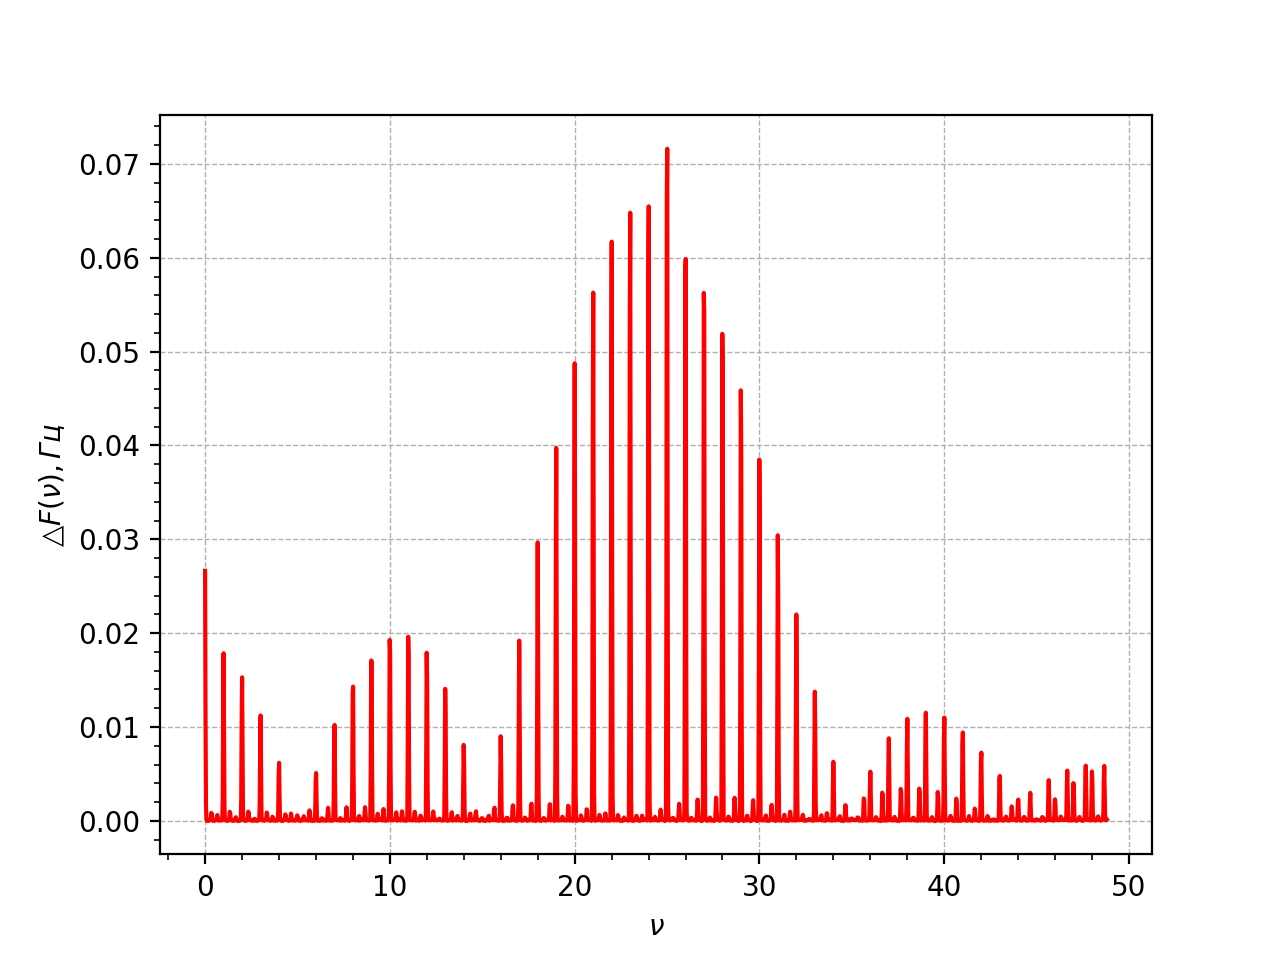
\includegraphics[width=\linewidth]{4.png}\\
\begin{center}
Рис.15 "Эталонный спектр"
\end{center}
\end{minipage}
\begin{minipage}{0.1\textwidth}
\ \ \ \ \ \ \Rightarrow
\end{minipage}
\begin{minipage}{0.44\textwidth}
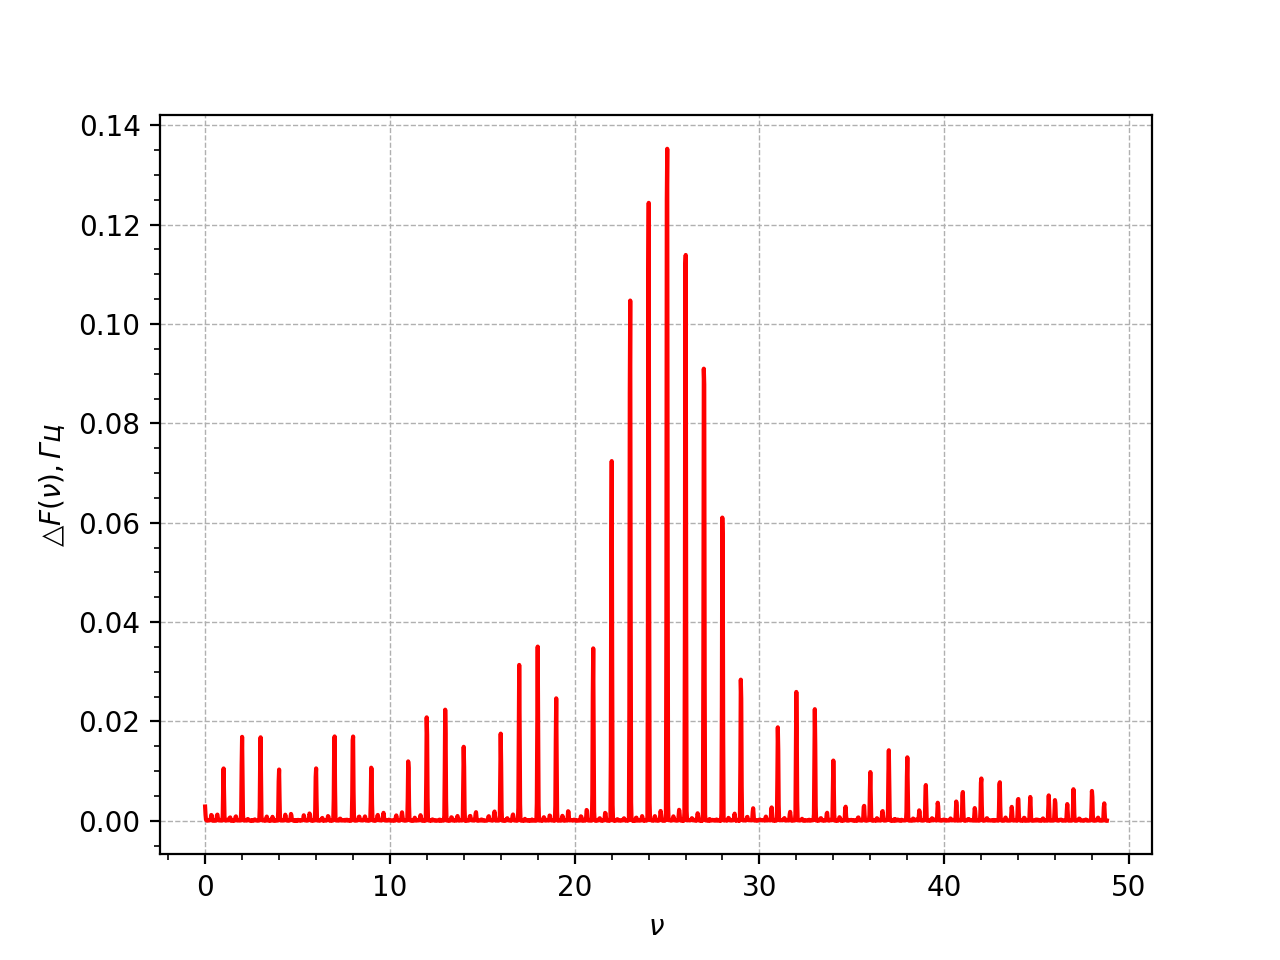
\includegraphics[width=\linewidth]{5.png}\\
\begin{center}
Рис.16 "Увеличение $\tau$ вдвое"
\end{center}
\end{minipage}

\\
\
\\


б) при изменении частоты несущей: $\nu_{0}=25,10$ или 40 кГц. изменяется только положение пика. \\

\begin{minipage}{0.3\textwidth}
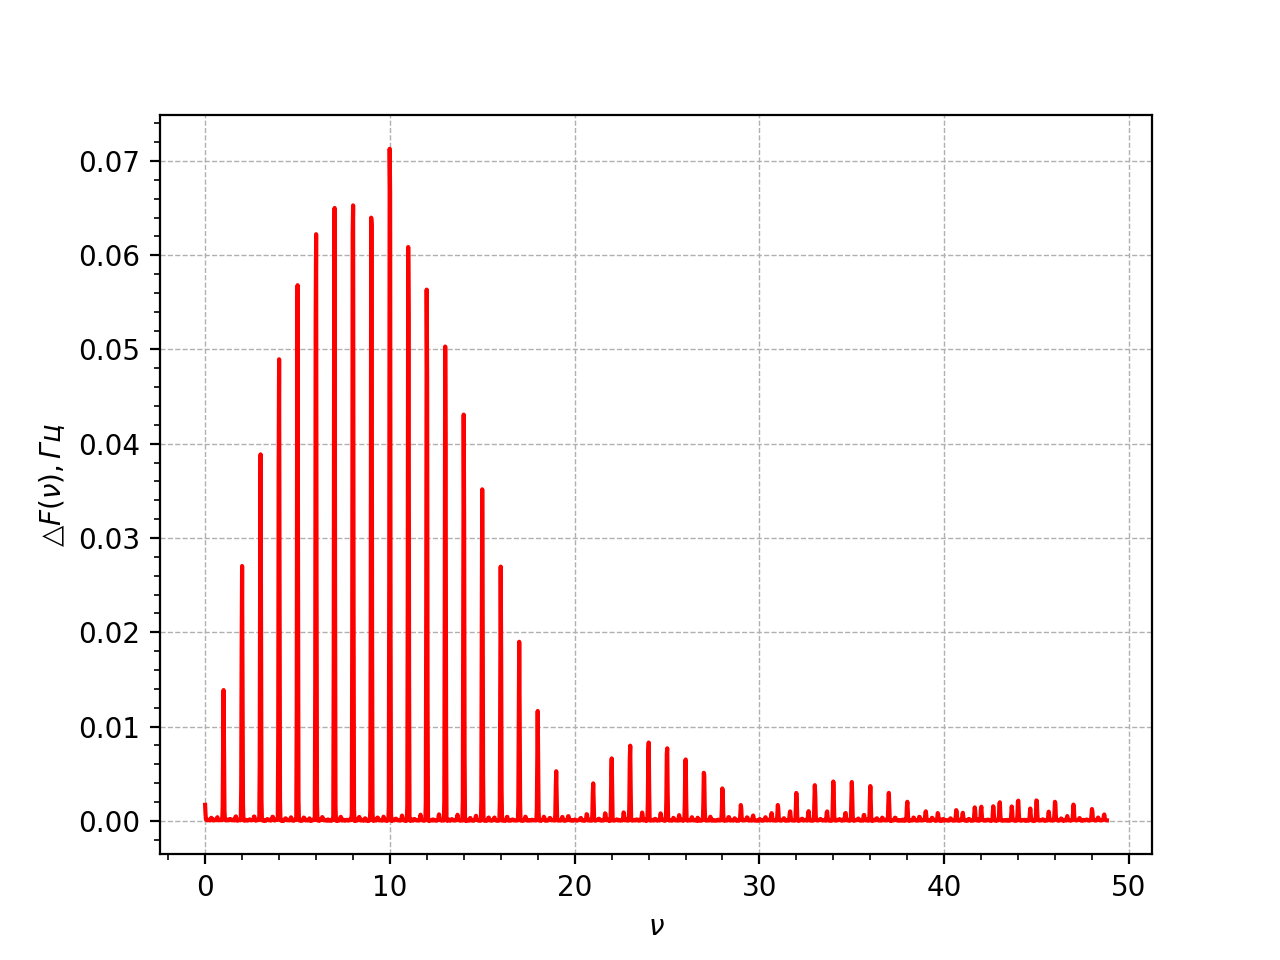
\includegraphics[width=\linewidth]{6.png}\\
\begin{center}
\ \ \ \ \ \ \ \ \ \ \ \ \nu_{0}=10 \ кГц
\end{center}
\end{minipage}
\begin{minipage}{0.05\textwidth}
\begin{center}
\ \ \Rightarrow
\end{center}
\end{minipage}
\begin{minipage}{0.3\textwidth}
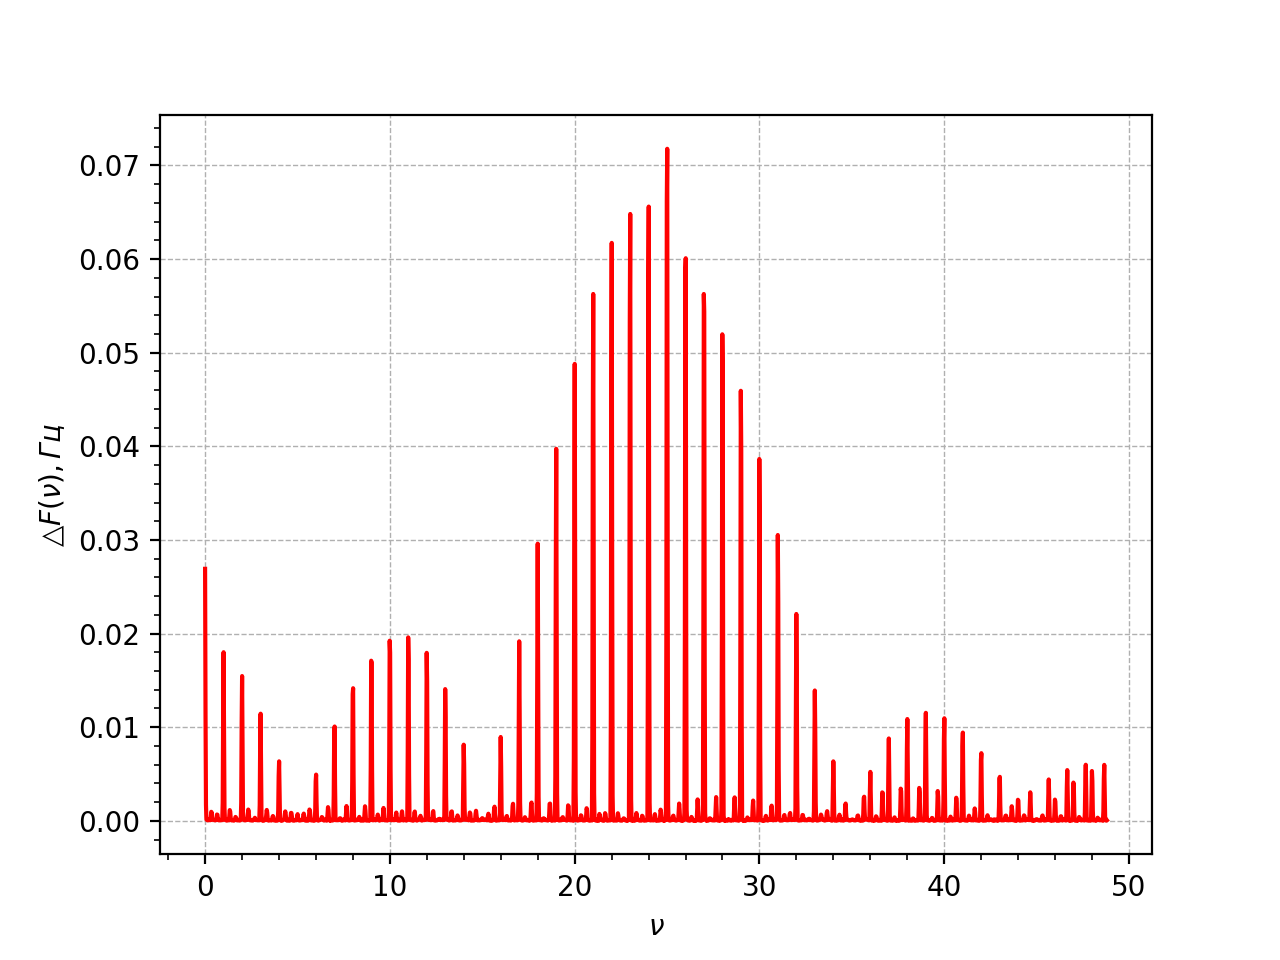
\includegraphics[width=\linewidth]{7.png}\\
\begin{center}
\ \ \ \ \ \ \ \ \ \ \ \ \nu_{0}=25 \ кГц
\end{center}
\end{minipage}
\begin{minipage}{0.05\textwidth}
\begin{center}
\ \ \Rightarrow
\end{center}
\end{minipage}
\begin{minipage}{0.3\textwidth}
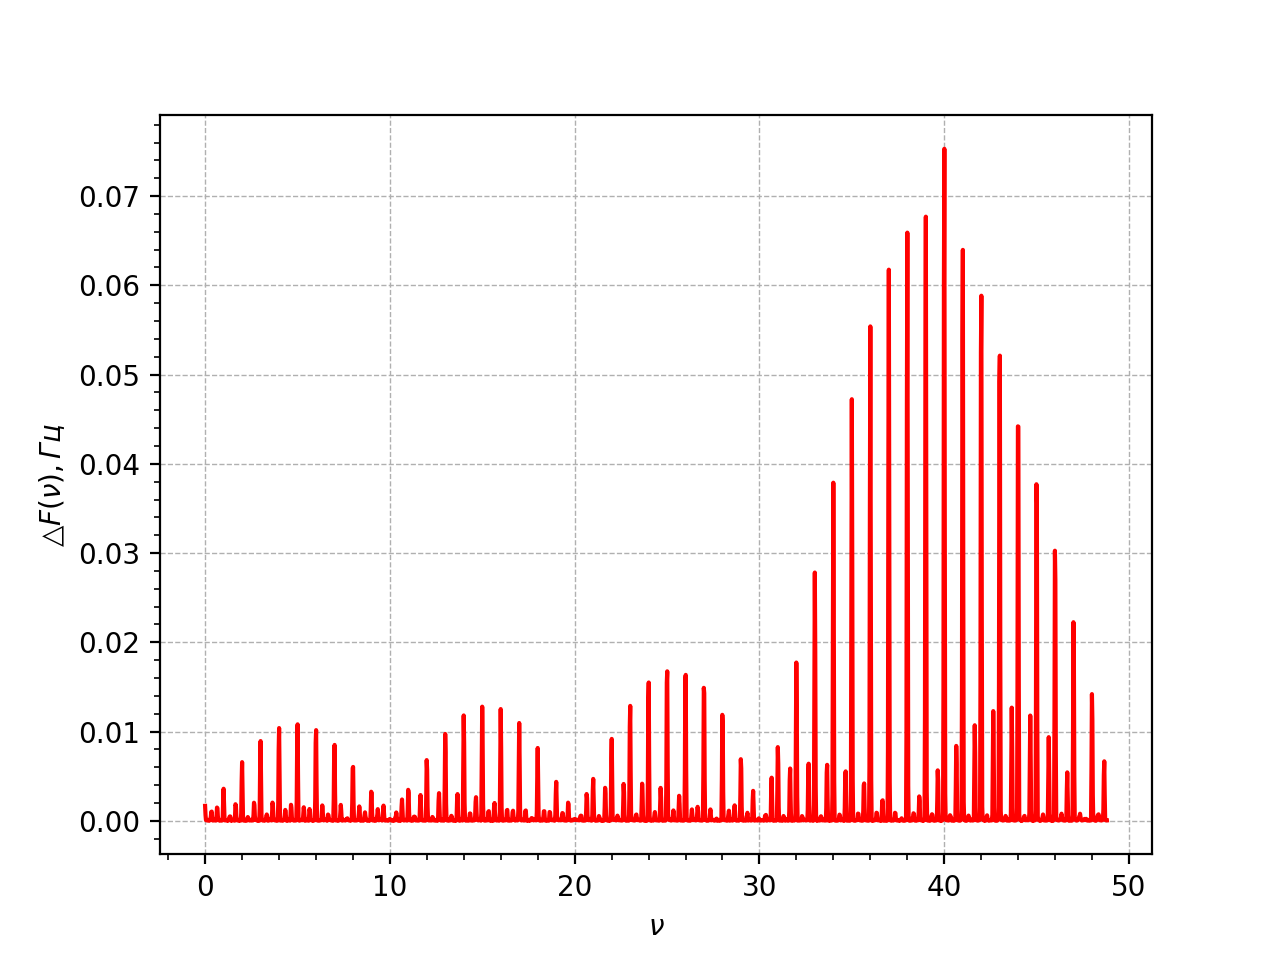
\includegraphics[width=\linewidth]{8.png}\\
\begin{center}
\ \ \ \ \ \ \ \ \ \ \ \ \nu_{0}=40 \ кГц
\end{center}
\end{minipage}

\begin{center}
{Рис.17} "Увеличение частоты несущей"
\end{center}
\\
\
\\
\

При фиксированной длительности импульсов $\tau=100$ мкс исследуем зависимость расстояния $\delta \nu$ между соседними спектральными компонентами от частоты повторения импульсов $f_{\text {повт }}$ в диапазоне $0,5-5 кГц$.

\begin{center}
\begin{tabular}{|c|c|}
\hline
$\delta \nu$, кГц & $f_{\text {повт }}$, кГц \\ \hline
0,5 & 0,5 \\ \hline
1 & 1 \\ \hline
2 & 2 \\ \hline
4 & 4 \\ \hline
5 & 5 \\ \hline
\end{tabular}\\
{Таблица 2.} Зависимость $\delta \nu(f_{\text {повт }})$
\end{center}

\begin{center}
                    \begin{tikzpicture}
                        \begin{axis}[
                            title =  $ \delta \nu (f_{\text {повт }}) $ ,
                            grid = major,
                            height = 0.25\paperheight, 
                	        width = 0.7\paperwidth,
                            axis lines = middle,
            	            xlabel = {$f_{\text {повт }}$, кГц },
            	            ylabel = {$\delta \nu$, кГц},
            	            xmin = 0,
            	            xmax = 7,
            	            ymin = 0,
                            ymax = 7
                        ]
                        \addplot[only marks,
                            x dir=both, x explicit,
                            y dir=both, y explicit,] 
                            table [y] {
                                x       y 
                                0.5	    0.5
                                1       1
                                2	    2
                                4       4
                                5       5     
                            };
                        \addplot[draw = red] coordinates {
            	            (0, 0) (7, 7)
                        };
                        \end{axis}
                    \end{tikzpicture} 
                    \begin{center}
                    {Рис 18.} График зависимости расстояния между соседними спектральными компонентами от частоты повторения импульса\\
                    \end{center}
                \end{center}
Угловой коэффициент полученной зависимости $k$ = 1, что совпадает с теоретическим.\\
                Построим картины спектров для $f_{\text {повт }}$  =  1 кГц  (рис. 19) и $ f$ = 2 кГц  (рис. 20).

\begin{figure}[p]
	\centering
	\includegraphics[width=0.8\linewidth]{"f1"}
                     \begin{center}
                    {Рис 19.} Картина спектра цугов при $f_{\text {повт }}$ = 1 кГц\\
                    \end{center}

	\label{fig:1-50}
\end{figure}

\begin{figure}[p]
	\centering
	\includegraphics[width=0.8\linewidth]{"f2"}
 \begin{center}
                    {Рис 20.} Картина спектра цугов при $f_{\text {повт }}$ = 2 кГц\\
                    \end{center}
	\label{fig:1-100}
\end{figure}

\newpage
Сравним спектры цугов и прямоугольных импульсов при одинаковых значениях $\tau$ и $T$:


\begin{minipage}{0.45\textwidth}
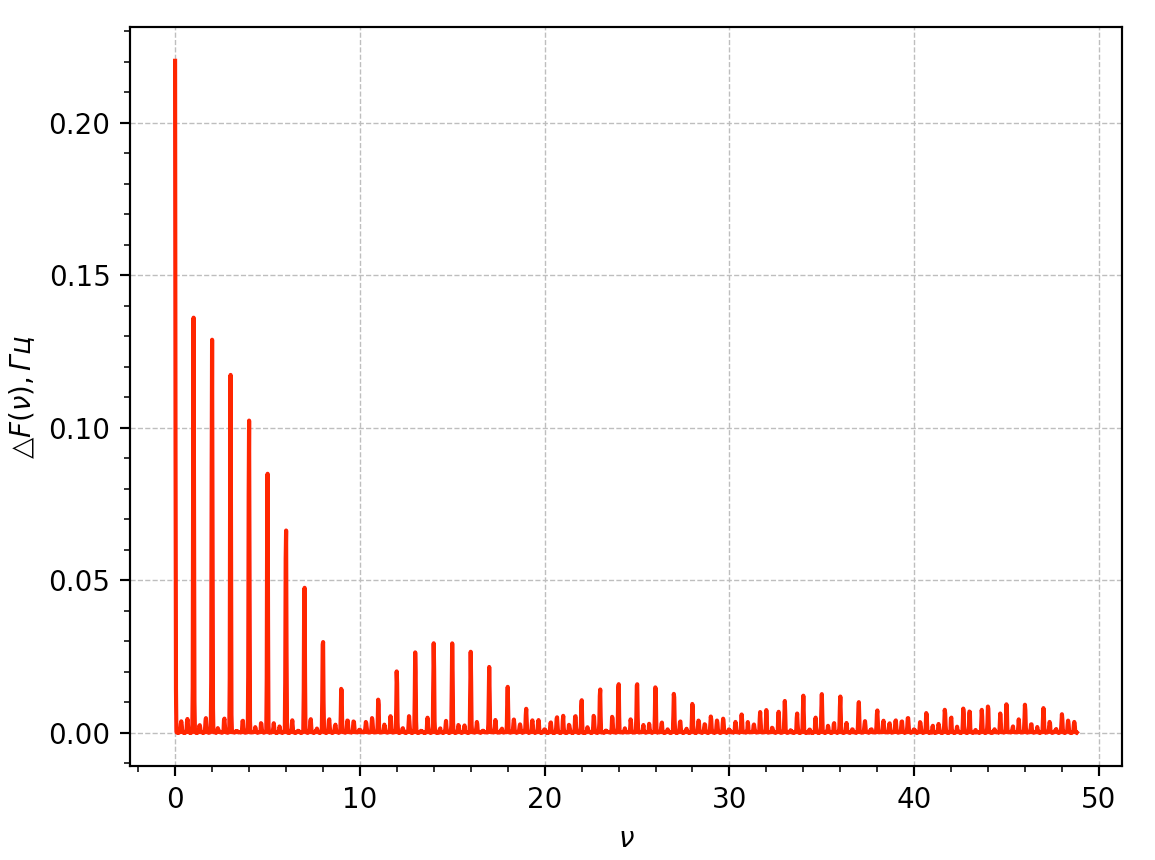
\includegraphics[width=\linewidth]{1.png}\\
\begin{center}
Спектр цугов при $\tau = 100 \ мкс $ и $T = 10^{-3} \ c$
\end{center}
\end{minipage}
\begin{minipage}{0.05\textwidth}
\
\end{minipage}
\begin{minipage}{0.45\textwidth}
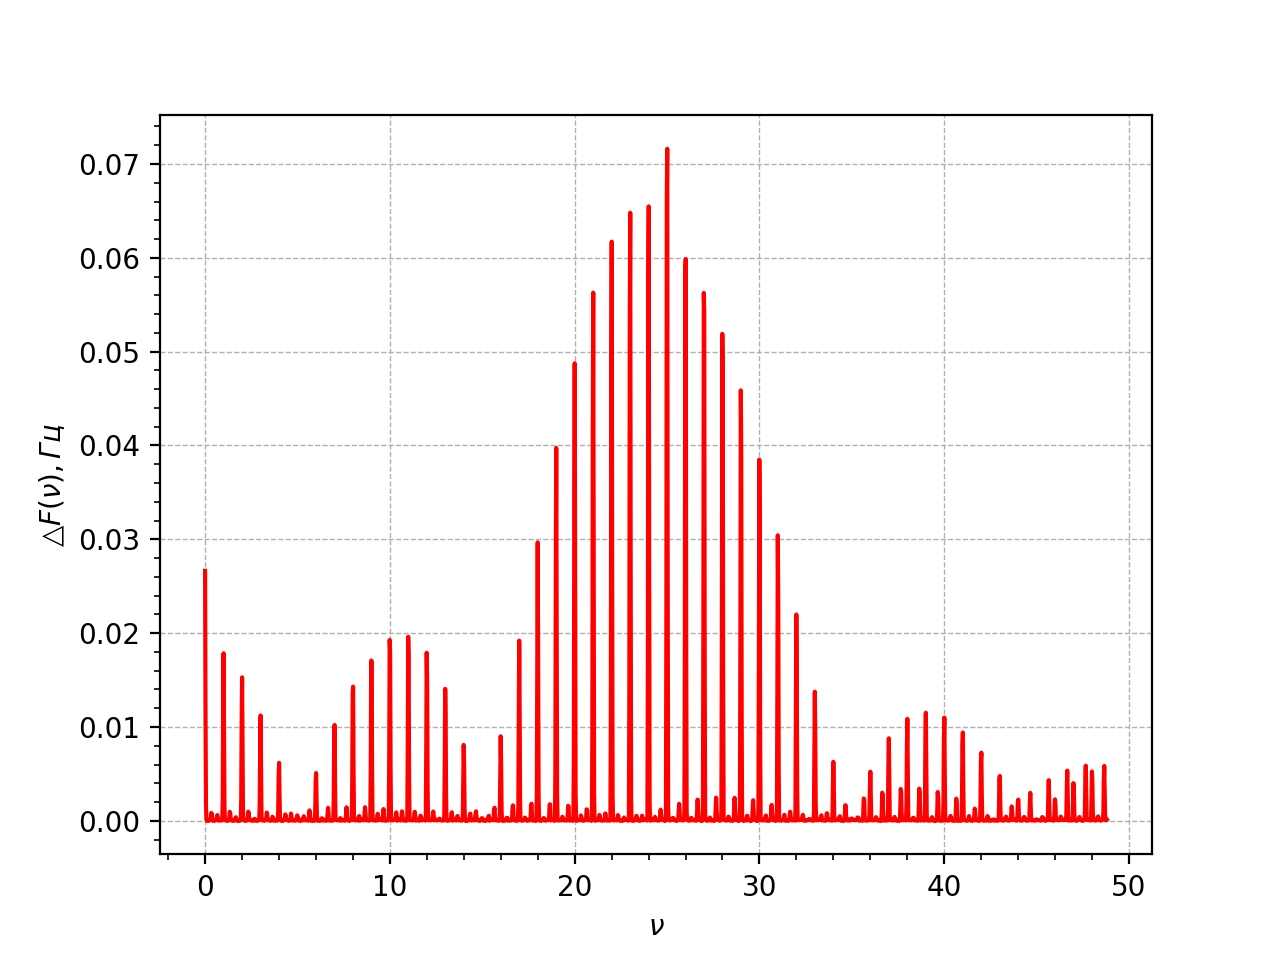
\includegraphics[width=\linewidth]{4.png}\\
\begin{center}
Спектр прямоугольных импульсов при $\tau = 100 \ мкс $ и $T = 10^{-3} \ c$
\end{center}
\end{minipage}


\\
\
\\
\

Явные отличия -- положение пиков и величина амплитуды. 

\subsection{Спектры гармонических колебаний, модулированных по амплитуде}

В этой части исследуется зависимость отношения амплитуд спектральных линий синусоидального сигнала, модулированного низкочастотными гармоническими колебаниями, от коэффициента модуляции, который определяется с помощью осциллографа.

Изменяя глубину модуляции, исследуем зависимость отношения амплитуды боковой линии спектра к амплитуде основной линии $\left(A_{\text {бок }} / A_{\text {осн }}\right)$ от глубины модуляции $m ;$ для расчёта глубины модуляции $m$ измерим максимальную $2 A_{\max }$ и минимальную $2 A_{\min }$ амплитуды сигнала на экране осциллографа. 

\begin{center}
\begin{tabular}{|c|c|c|c|c}
\hline
$2A$, В & $2 A_{\max }$, мВ & $2 A_{\min }$, мВ  & $A_{\text {бок }}$, мВ &  $A_{\text {осн }}$, мВ\\ \hline
0,2 & 444,8 & 555,7 & 16,6 & 323,5 \\ \hline
0,5 & 378,3 & 614,9 & 41,59 & 323,5 \\ \hline
0,8 & 297 & 696 & 62,8 & 323,5\\ \hline
1,1 & 230 & 770 & 87 & 323,5\\ \hline
1,4 & 142 & 822 & 112 & 323,5\\ \hline
1,7 & 83 & 918 & 134 & 323,5\\ \hline
2 & 23,38 & 992 & 166 & 323,5\\ \hline
\end{tabular}\\
{Таблица 3.} Зависимость $\left(A_{\text {бок }} / A_{\text {осн }}\right)$ от глубины модуляции $m
\end{center}

\begin{center}
                    \begin{tikzpicture}
                        \begin{axis}[
                            title =   $\left(A_{\text {бок }} / A_{\text {осн }}\right)(m)$ ,
                            grid = major,
                            height = 0.25\paperheight, 
                	        width = 0.7\paperwidth,
                            axis lines = middle,
            	            xlabel = {$\left(A_{\text {бок }} / A_{\text {осн }}\right)$ },
            	            ylabel = {$m$},
            	            xmin = 0,
            	            xmax = 1,
            	            ymin = 0,
                            ymax = 1
                        ]
                        \addplot[only marks,
                            x dir=both, x explicit,
                            y dir=both, y explicit,] 
                            table [y] {
                                x           y 
                                0.110       0.05
                                0.238       0.13       
                                0.401       0.19
                                0.54        0.26
                                0.705       0.34        
                                0.834       0.41
                                0.953       0.51
                            };
                        \addplot[draw = red] coordinates {
            	            (0, 0) (1, 0.5)
                        };
                        \end{axis}
                    \end{tikzpicture} 
                    \begin{center}
                    {Рис 18.} График зависимости отношения амплитуды боковой линии спектра к амплитуде основной линии от глубины модуляции\\
                    \end{center}
                \end{center}

Из графика
$$\frac{\left(A_{\text {бок }} / A_{\text {осн }}\right)}{m} = 0.522\pm0.015,$$
что сходится с теоретическим значением $0.5$.

\subsection{Спектр гармонических сигналов модулированных по частоте}

При 100\% глубине модуляции при $f_{\text{мод}}$ = 2 кГц расстояние между пиками увеличилось в 2 раза(т.е. в 2 раза увеличилась частота модуляции).Период модулирования сигнала уменьшился в 2 раза.

\section{Обсуждение результатов и выводы}

Исследования зависимости ширины спектра периодической последовательности прямоугольных импульсов от длительности отдельного импульса в первой части работы полностью совпали с теоретическими рассчетами. По наклону графика из этой части можно убедиться в соотношении неопределенностей ($\quad \Delta \nu \Delta t \simeq 1$).
 
Исследования зависимости расстояния между ближайшими спектральными компонентами от частоты повторения цугов дали схожие результаты. 

В последней части коэффициенты, получаемые в результате исследования зависимости отношения амплитуд спектральных линий синусоидального сигнала, модулированного низкочастотными гармоническими колебаниями, от коэффициента модуляции полностью совпали с теоретически рассчитаными. 



\end{document}